	\documentclass[11pt,a5paper]{article}
\usepackage[utf8]{inputenc}
\usepackage[english]{babel}
\usepackage{amsmath}
\usepackage{amsthm}
\usepackage{amsfonts}
\usepackage[margin=0.47in]{geometry}
\usepackage{graphicx}

\newtheorem{theorem}{Example}
\newtheorem{exercise}{Exercise}
\newtheorem*{Theorem}{Theorem}

\title{\textbf{Geometry I.}}
\date{Week 8}
\author{Miroslav Stankovic\\ Marko Puza}
\begin{document}
\maketitle

\section{Theory}

\noindent One of the most beautiful (I might be biased here) topics in problem solving is Euclidean geometry. In this sheet we will briefly iterate over some well-known theorems and look in more detail into properties of cyclic quadrilaterals.

\subsection*{Basic theorems}

\begin{Theorem}[Parallel liness]
	In the figure 1 below, the lines $x$ and $y$ are parallel. Then we have  $a=c=g=e$, $b=d=f=h$, and $b+g = 180^{\circ}$.
\end{Theorem}

\begin{figure}[h] \begin{center}
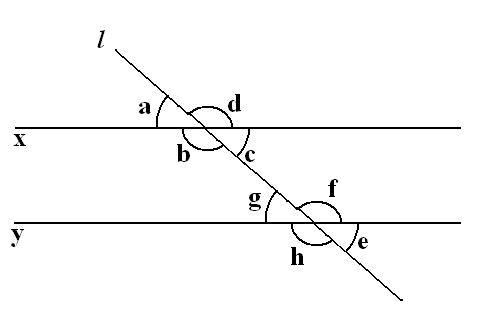
\includegraphics[width=0.5\textwidth]{parallel}
\caption{Parallel lines}
\end{center} \end{figure}

\begin{exercise} In the figure 1, $a=3x-33^{\circ}$ and $h=7x+3^{\circ}$. Find $x$.
\end{exercise}


\begin{figure}[h] \begin{center}
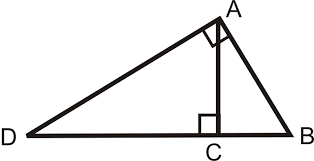
\includegraphics[width=0.5\textwidth]{right}
\caption{Parallel lines}
\end{center} \end{figure}

\begin{Theorem}[Pythagorean]
	In the right-angled triangle (figure 2), $AB^2 + AD^2 = BD^2$.
\end{Theorem}
\begin{Theorem}[Thales']
	$BD$ is a diameter of circumcircle of $\triangle ABD$.
\end{Theorem}
\begin{Theorem}[Geometric mean theorem]
	Altitude Rule: $CA^2 = CD \cdot CB$.\\
	Leg Rule:  $BA^2 = BC \cdot BD$.
\end{Theorem}
\begin{exercise} Prove \emph{Geometric mean theorem} (both rules).
\end{exercise}

\subsection*{Cyclic quadrilaterals}

Lorem ipsum...

\section{Problems}


\begin{enumerate}
	\subsection*{Easy}
	
	\subsection*{Medium}	
	
	\subsection*{Difficult}

	\subsection*{Extra}	
	\item{Blah.}

\end{enumerate}

\begin{thebibliography}{9}
\bibitem{KMS} Ondrej Budáč, Tomáš Jurík, and Ján Mazák. 
	\emph{Zbierka úloh KMS}. Trojsten, Bratislava, 2010.
	
\bibitem{PraSe} Matematický korespondenční seminář. Knihovna. [ONLINE] Available at: \texttt{https://mks.mff.cuni.cz/library/library.php}. [Accessed 10 October 26].
\end{thebibliography}

\section{Hints}
\begin{enumerate}
	\subsection*{Easy}
	\subsection*{Medium}
	\subsection*{Difficult}
	\subsection*{Extra}	
	\item{Blah blah.)}
\end{enumerate}
\end{document}
